\documentclass[12pt, a4paper, oneside]{ctexart}
\usepackage{amsmath, amsthm, amssymb, bm, color, graphicx, geometry, mathrsfs,extarrows, braket, booktabs, array}
\usepackage[colorlinks,linkcolor=red,anchorcolor=blue,citecolor=blue,urlcolor=blue,menucolor=black]{hyperref}
%%%% 设置中文字体 %%%%
\setCJKmainfont{方正新书宋_GBK.ttf}[BoldFont=方正小标宋_GBK, ItalicFont=方正楷体_GBK]
%%%% 设置英文字体 %%%%
\setmainfont{Times New Roman}
\setsansfont{Calibri}
\setmonofont{Consolas}

\linespread{1.4}
%\geometry{left=2.54cm,right=2.54cm,top=3.18cm,bottom=3.18cm}
\geometry{left=1.84cm,right=1.84cm,top=2.18cm,bottom=2.18cm}
\newcounter{problem}  % 问题序号计数器
\newenvironment{problem}{\stepcounter{problem}\par\noindent\textbf{题目\arabic{problem}. }}{\smallskip\par}
\newenvironment{solution}[1][]{\par\noindent\textbf{#1解答. }}{\smallskip\par}  % 可带一个参数表示题号\begin{solution}{题号}
\newenvironment{note}{\par\noindent\textbf{注记. }}{\smallskip\par}

%%%% 图片相对路径 %%%%
\graphicspath{{figure/}} % 当前目录下的figure文件夹, {../figure/}则是父目录的figure文件夹
\setlength{\abovecaptionskip}{-0.2cm}  % 缩紧图片标题与图片之间的距离
\setlength{\belowcaptionskip}{0pt} 

\everymath{\displaystyle} % 默认全部行间公式
\DeclareMathOperator*\uplim{\overline{lim}} % 定义上极限 \uplim_{}
\DeclareMathOperator*\lowlim{\underline{lim}} % 定义下极限 \lowlim_{}
\DeclareMathOperator*{\argmax}{arg\,max}  % \argmin
\DeclareMathOperator*{\argmin}{arg\,min}  % \argmax
\let\leq=\leqslant % 将全部leq变为leqslant
\let\geq=\geqslant % geq同理

%%%% 一些宏定义 %%%%
\def\bd{\boldsymbol}        % 加粗(向量) boldsymbol
\def\disp{\displaystyle}    % 使用行间公式 displaystyle(默认)
\def\tsty{\textstyle}       % 使用行内公式 textstyle
\def\sign{\text{sign}}      % sign function
\def\wtd{\widetilde}        % 宽波浪线 widetilde
\def\R{\mathbb{R}}          % Real number
\def\N{\mathbb{N}}          % Natural number
\def\Z{\mathbb{Z}}          % Integer number
\def\Q{\mathbb{Q}}          % Rational number
\def\C{\mathbb{C}}          % Complex number
\def\N{\mathbb{N}}          % Natural number
\def\Z{\mathbb{Z}}          % Integer number
\def\E{\mathbb{E}}          % Exception
\def\var{\text{Var}}        % Variance
\def\bias{\text{bias}}      % bias
\def\d{\mathrm{d}}          % differential operator
\def\e{\mathrm{e}}          % Euler's number
\def\i{\mathrm{i}}          % imaginary number
\def\re{\mathrm{Re}}        % Real part
\def\im{\mathrm{Im}}        % Imaginary part
\def\res{\mathrm{Res}}      % Residue
\def\L{\mathcal{L}}         % Loss function
\def\wdh{\widehat}          % 宽帽子 widehat
\def\ol{\overline}          % 上横线 overline
\def\ul{\underline}         % 下横线 underline
\def\add{\vspace{1ex}}      % 增加行间距
\def\del{\vspace{-1.5ex}}   % 减少行间距

%%%% 定理类环境的定义 %%%%
\newtheorem{theorem}{定理}

%%%% 基本信息 %%%%
\newcommand{\RQ}{\today} % 日期
\newcommand{\km}{数理统计} % 科目
\newcommand{\bj}{强基数学002} % 班级
\newcommand{\xm}{吴天阳} % 姓名
\newcommand{\xh}{2204210460} % 学号
\newcommand{\id}{50} % 序号

\begin{document}

%\pagestyle{empty}
\pagestyle{plain}
\vspace*{-15ex}
\centerline{\begin{tabular}{*6{c}}
    \parbox[t]{0.25\linewidth}{\begin{center}\textbf{日期}\\ \large \textcolor{blue}{\RQ}\end{center}} 
    & \parbox[t]{0.2\linewidth}{\begin{center}\textbf{科目}\\ \large \textcolor{blue}{\km}\end{center}}
    & \parbox[t]{0.2\linewidth}{\begin{center}\textbf{班级}\\ \large \textcolor{blue}{\bj}\end{center}}
    & \parbox[t]{0.1\linewidth}{\begin{center}\textbf{姓名}\\ \large \textcolor{blue}{\xm}\end{center}}
    & \parbox[t]{0.15\linewidth}{\begin{center}\textbf{学号}\\ \large \textcolor{blue}{\xh}\end{center}}
    & \parbox[t]{0.1\linewidth}{\begin{center}\textbf{序号}\\ \large \textcolor{blue}{\id}\end{center}}
     \\ \hline
\end{tabular}}
\begin{center}
    \zihao{3}\textbf{第三次作业}
\end{center}\vspace{-0.2cm}
\begin{problem}
    设$X_1,\cdots, X_n$是来自某一个分布的随机样本,期望为$\mu$方差为$\sigma^2$.

    1. 证明$\sum_{i=1}^na_iX_i$是$\mu$的无偏估计,其中$\sum_{i=1}^na_i=1$.

    2. 若$\sum_{i=1}^na_i=1$,证明当$a_i=\frac{1}{n},\ (i=1,2,\cdots,n)$时,$\var\left(\sum_{i=1}^na_i\right)$取到最小值.
\end{problem}
\begin{proof}
    1. $\E\left(\sum_{i=1}^na_iX_i\right) = \sum_{i=1}^na_i\E(X_i) = \mu\sum_{i=1}^na_i=\mu$,于是$\bias\left(\sum_{i=1}^na_iX_i\right) = \E\left(\sum_{i=1}^na_iX_i\right)-\mu = 0$,所以$\sum_{i=1}^na_iX_i$是无偏估计.\add

    2. \ \del
    \begin{align*}
        \var\left(\sum_{i=1}^na_iX_i\right) =&\  \E\left(\left(\sum_{i=1}^na_iX_i\right)^2\right) - \mu^2 = (\sigma^2+\mu^2)\sum_{i=1}^na_i^2+2\mu^2\sum_{1\leq i<j\leq n}a_ia_j - \mu^2\\
        =&\ \sigma^2\sum_{i=1}^na_i^2+\mu^2\left(\sum_{i=1}^na_i^2+2\sum_{1\leq i < j\leq n}a_ia_j-1\right)\\
        =&\ \sigma^2\left(\sum_{i=1}^n\left(a_i-\frac{1}{n}\right)^2+\frac{1}{n}\right)+\mu^2\left(\left(\sum_{i=1}^na_i\right)^2-1\right)\\
        =&\ \sigma^2\left(\sum_{i=1}^n\left(a_i-\frac{1}{n}\right)^2+\frac{1}{n}\right)
    \end{align*}
    所以当$a_i = \frac{1}{n}$时,$\var\left(\sum_{i=1}^na_i\right)$取到最小值.
\end{proof}
\begin{problem}
    设$X_1,X_2,\cdots,X_n$是来自$f(x;\theta) = \frac{\theta}{x^2}I_{[\theta, \infty)}(x)$的随机变量,其中$\theta > 0$.

    1. 求$\theta$的MLE.

    2. $Y_1=\min\{X_1,\cdots, X_n\}$是充分统计量么?
\end{problem}
\begin{solution}
    1. 
    \begin{equation*}
        \L(\theta) = \prod_{i=1}^nf(x_i;\theta) = \prod_{i=1}^n\frac{\theta}{x_i^2}I_{[\theta,\infty)}(x_i) = \frac{\theta^n}{\prod_{i=1}^nX_i^2}I_{(-\infty, y_1]}(\theta)
    \end{equation*}
    所以$\hat{\theta} = Y_1$.

    2. 由于$\prod_{i=1}^nf(x_i;\theta) = \frac{\theta^n}{\prod_{i=1}^nx_i^2}I_{(-\infty, \theta]}(y_1)$,令
    \begin{equation*}
        S = Y_1,\ g(s;\theta) = \theta^2I_{(-\infty, \theta]}(y_1),\ h(x_1,\cdots, x_n)=\left(\prod_{i=1}^nx_i^2\right)^{-1}   
    \end{equation*}
    则$\prod_{i=1}^nf(x_i;\theta) = g(s;\theta)h(x_1,\cdots, x_n)$,由因子分解定理可知$Y_1$是充分统计量.
\end{solution}
\begin{problem}
    设$X_1,\cdots,X_n$是来自$f(x;\theta)=\frac{1}{\theta}I_{[0,\theta]}(x)$的随机变量,其中$\theta > 0$,定义$Y_n = \max\{X_1,\cdots, X_n\}, Y_1=\min\{X_1,\cdots, X_n\}$.

    1, 2. 对$\theta$分别求解矩估计$T_1$,最大似然估计$T_2$,并分别计算期望和均方误差.

    3. 对于所有形式为$aY_n$的估计量,其中$a$是依赖于$n$的常数,其中具有最小的均方误差记为$T_3$,求出$T_3$并计算期望和均方误差.

    4. 令$T_4 = Y_1+Y_n$,求出$T_4$的期望和均方误差.

    5. 如何确定哪个估计量最优.

    6. 求关于总体方差的MLE.
\end{problem}
\begin{solution}
    1. 矩估计:$\bar{X} = E(X) = \frac{\theta}{2}\Rightarrow T_1 = 2\bar{X}$. 期望:$\E(T_1) = \E(2\bar{X}) = \theta$,所以$T_1$是无偏估计.  均方误差:$\text{MSE}(T_1) = \var(T_1) = 4\frac{\var(X)}{n} = \frac{\theta^2}{3n}$.\add

    2. MLE:$\L(\theta) = \prod_{i=1}^nf(x_i;\theta) = \frac{1}{\theta^n}\prod_{i=1}^nI_{[0,\theta]}(x_i) = \frac{1}{\theta^n}I_{[y_n,\infty)}(\theta)I_{[0,y_n]}(y_1)$,则$T_2 = Y_n$.
    
    由于$f_{Y_n}(x) = nF_X(x)^{n-1}f_X(x)  = n\frac{x^{n-1}}{\theta^n}I_{[0,\theta]}(x)$,于是$T_2$的期望为
    \begin{align*}
        \E(T_2) =&\ \E(Y_n) = \int_0^\theta n\frac{x^n}{\theta^n}\,\d x = \frac{n}{n+1}\theta,\\
        \E(T_2^2) =&\ \E(Y_n^2) = \int_0^\theta n\frac{x^{n+1}}{\theta^n}\,\d x = \frac{n}{n+2}\theta^2.
    \end{align*}
    均方误差:$\text{MSE}(T_2) = \E((T_2-\theta)^2) = \E(T_2^2)-2\theta\E(T_2)+\theta^2 = \frac{2}{(n+1)(n+2)}\theta^2$.\add

    3. 设$T_3 = aY_n$,由第二问可知$\E(T_3) = \frac{an}{n+1}\theta,\ \E(T_3^2) = \frac{a^2n}{n+2}\theta^2$,则
    \begin{equation*}
        \text{MSE}(T_3) = \frac{a^2n}{n+2}\theta^2-\frac{2an}{n+1}\theta^2+\theta^2 = \frac{a^2n(n+1)-2an(n+2)+(n+1)(n+2)}{(n+1)(n+2)}\theta^2.
    \end{equation*}
    令$\varphi(a) =a^2n(n+1)-2an(n+2)+(n+1)(n+2)$,则$\varphi'(a_0) = 0\Rightarrow a_0 = \frac{n+2}{n+1}$,所以$T_3 = \frac{n+2}{n+1}Y_n$,对应的期望和均方误差分别为
    \begin{align*}
        \E(T_3) = \frac{n+2}{n+1}\E(T_2) = \frac{n(n+2)}{(n+1)^2}\theta,\quad
        \text{MLE}(T_3) = \frac{\theta^2}{(n+1)^2}.
    \end{align*}

    4. 由次序统计量的性质可知$f_{Y_1,Y_n} = \frac{n(n-1)(y_n-y_1)^{n-2}}{\theta^n},\ (0\leq y_1\leq y_n\leq \theta)$,于是
    \begin{align*}
        \E(Y_1Y_n)=&\ \int_0^\theta\int_{y_1}^\theta y_1y_n\frac{n(n-1)(y_n-y_1)^{n-2}}{\theta^n}\,\d y_n\,\d y_1\\
        \xlongequal{x=y_n-y_1}&\ \frac{n(n-1)}{\theta^n}\int_0^\theta y_1\int_0^{\theta-y_1}(x+y_1)x^{n-2}\,\d x\,\d y_1\\
        =&\ \frac{n(n-1)}{\theta^n}\int_0^\theta y_1\left(\frac{(\theta-y_1)^n}{n}+\frac{y_1(\theta-y_1)^{n-1}}{n-1}\right)\,\d y_1\\
        \xlongequal{y=\theta-y_1}&\ \frac{n(n-1)}{\theta^n}\int_0^\theta\left((\theta-y)\frac{y^n}{n}+(\theta-y)^2\frac{y^{n-1}}{n-1}\right)\d y\\
        =&\ \frac{n(n-1)}{\theta^n}\left(\frac{1}{n(n+1)}-\frac{1}{n(n+2)}+\frac{1}{n(n-1)}-\frac{2}{(n+1)(n-1)}+\frac{1}{(n+2)(n-1)}\right)\theta^{n+2}\\
        =&\ \frac{\theta^2}{n+2},
    \end{align*}
    由于$f_{Y_1} = \frac{n}{\theta}(1-\frac{y_1}{\theta})^{n-1}$,则
    \begin{align*}
        \E(Y_1) =&\ \int_0^{\theta}\frac{n}{\theta}y_1\left(1-\frac{y_1}{\theta}\right)^{n-1}\,\d y_1
        \xlongequal{\theta(1-x)=y_1} \theta n\int_0^{1}(x^{n-1}-x^n)\,\d x
        = \frac{\theta}{n+1},\\
        \E(Y_n) =&\ \int_0^\theta\frac{n}{\theta}y_1^2\left(1-\frac{y_1}{\theta}\right)^{n-1}\,\d y_1
        \xlongequal{\theta(1-x) = y_1} \theta^2n\int_0^1(1-x)^2x^{n-1}\,\d x
        = \frac{2}{(n+1)(n+2)}\theta^2,
    \end{align*}
    由第二小问可知$\E(Y_n) = \frac{n}{n+1}\theta,\ \E(Y_n^2) = \frac{n}{n+2}\theta^2$,于是
    \begin{align*}
        \E(T_4)=&\ \E(Y_1+Y_n) = \E(Y_1)+\E(Y_n) = \frac{\theta}{n+1}+\frac{n}{n+1}\theta = \theta,\ \text{(所以}T_4\text{是无偏估计)}\\
        \E(T_4^2) =&\ \E(Y_1^2)+2\E(Y_1Y_n)+\E(Y_n^2) = \frac{n^2+3n+4}{(n+1)(n+2)}\theta^2,\\
        \text{MSE}(T_4) =&\ \var(T_4) = \E(T_4^2)-\E(T_4)^2 = \frac{n^2+3n+4}{(n+1)(n+2)}\theta^2-\theta^2 = \frac{2}{(n+1)(n+2)}\theta^2.
    \end{align*}

    5. $T_3$具有最小的MSE,所以$T_3$最优.

    6. 由于总体方差是关于$\theta$的函数,则其MLE为$\frac{\hat{\theta}^2}{12}$,其中$\hat{\theta}$为$\theta$的估计量.
\end{solution}
\begin{problem}
    设$X_1,\cdots,X_n$是来自均匀分布$U(\theta,2\theta),\ \theta>0$的样本,试给出充分统计量.
\end{problem}
\begin{solution}
    由于$f(x) = \frac{1}{\theta}I_{[\theta,2\theta]}(x)$,于是
    \begin{equation*}
        \prod_{i=1}^nf(x_i) = \frac{1}{\theta^n}\prod_{i=1}^nI_{[\theta,2\theta]}(x_i) = \frac{1}{\theta^n}I_{[\theta,y_n]}(y_1)I_{[y_1,2\theta]}(y_n),
    \end{equation*}
    所以$\theta$的充分统计量可以为$Y_1,Y_n$.
\end{solution}
\begin{problem}
    设$X_1,\cdots,X_n$是来自Gamma分布$\{\Gamma(a,\lambda):\alpha > 0,\lambda > 0\}$的样本,寻求$\alpha,\lambda$的充分统计量.
\end{problem}
\begin{solution}
    由于$f(x) = \frac{\lambda^\alpha}{\Gamma(\alpha)}x^{\alpha-1}\e^{-\lambda x}$,于是
    \begin{equation*}
        \prod_{i=1}^nf(x_i) = \frac{\lambda^{n\alpha}}{\Gamma(\alpha)^n}\left(\prod_{i=1}^nx_i\right)^{\alpha-1}\e^{-\lambda\sum\limits_{i=1}^nx_i}
    \end{equation*}
    所以$\alpha, \lambda$的充分统计量可以是$\sum_{i=1}^nX_i,\prod_{i=1}^nX_i$.
\end{solution}
\begin{problem}
    设$X_1,\cdots,X_n$是$N(\mu,\sigma_1^2)$的样本,$Y_1,\cdots, Y_m$是来自$N(\mu,\sigma_2^2)$的样本,这两个样本相互独立,试给出$\mu,\sigma_1^2,\sigma_2^2$的充分统计量.
\end{problem}
\begin{solution}
    由于$f_X(x) = \frac{1}{\sqrt{2\pi\sigma_1^2}}\e^{-\frac{(x-\mu)^2}{2\sigma_1^2}},\ f_Y(x) = \frac{1}{\sqrt{2\pi\sigma_2^2}}\e^{-\frac{(y-\mu)^2}{2\sigma_1^2}}$,于是
    \begin{align*}
        \prod_{i=1}^nf_X(x_i)\prod_{j=1}^mf_Y(y_j) =&\ \frac{1}{(2\pi\sigma_1^2)^{\frac{n}{2}}(2\pi\sigma_2^2)^{\frac{m}{2}}}\exp\left\{-\frac{\sum_{i=1}^n(x_i-\mu)^2}{2\sigma_1^2}-\frac{\sum_{j=1}^n(y_j-\mu)^2}{2\sigma_2^2}\right\}\\
        =&\ \frac{1}{(2\pi\sigma_1^2)^{\frac{n}{2}}(2\pi\sigma_2^2)^{\frac{m}{2}}}\exp\left\{-\frac{\sum_{i=1}^nx_i^2-2\mu\sum_{i=1}^nx_i+\mu^2}{2\sigma_1^2}-\frac{\sum_{j=1}^ny_j-2\mu\sum_{j=1}^my_j+\mu^2}{2\sigma_2^2}\right\}
    \end{align*}
    所以$\mu,\sigma_1^2,\sigma_2^2$的充分统计量可以为$\sum_{i=1}^nX_i^2,\sum_{i=1}^nX_i,\sum_{j=1}^mY_i^2,\sum_{j=1}^mY_i$.
\end{solution}

% 正文部分

% 下面给一些功能的写法
\iffalse
% 图片模板
\centerline{
    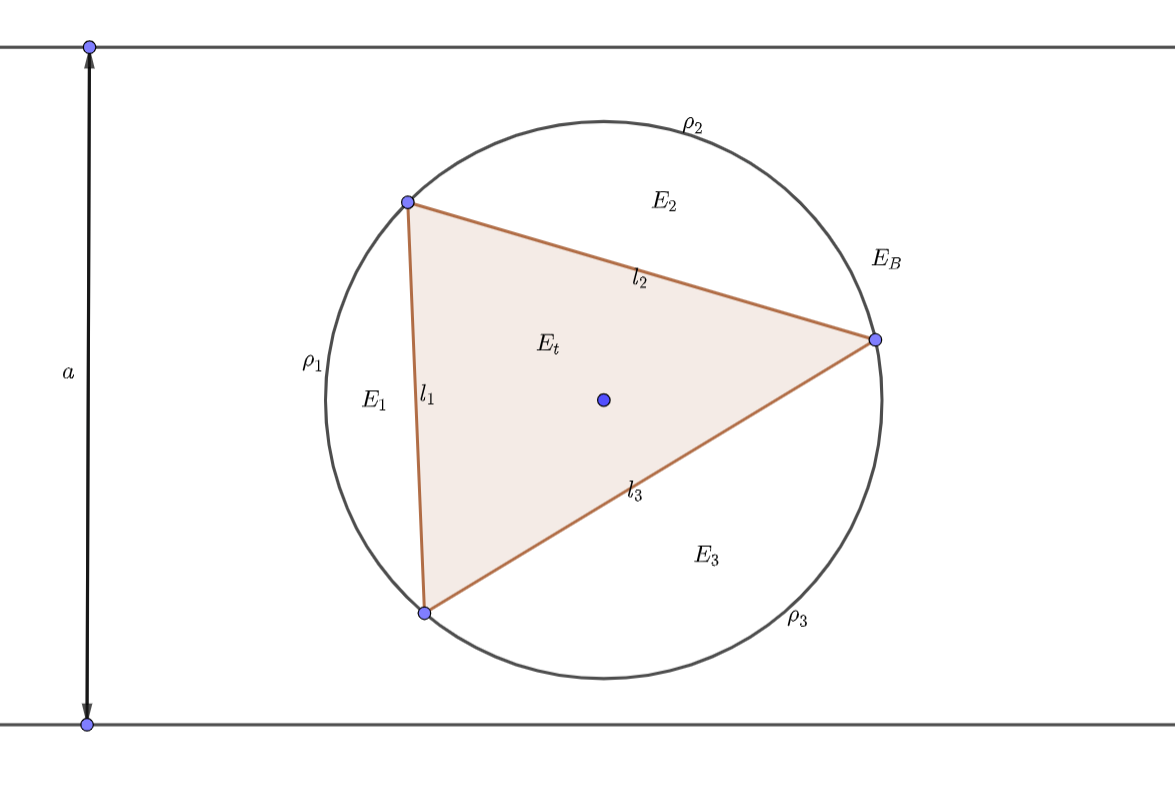
\includegraphics[width=0.8\textwidth]{figure.png}
}
% 表格模板
\renewcommand\arraystretch{0.8} % 设置表格高度为原来的0.8倍
\begin{table}[!htbp] % table标准
    \centering % 表格居中
    \begin{tabular}{p{1cm}<{\centering}p{1cm}<{\centering}p{3cm}<{\centering}p{5cm}<{\centering}} % 设置表格宽度
    %\begin{tabular}{cccc}
        \toprule
        $x_i$ & $f[x_1]$ & $f[x_i,x_{i+1}]$ & $f[x_i,x_{i+1},x_{i+2}]$ \\
        \midrule
        $x_0$ & $f(x_0)$ &                  &                          \\
        $x_0$ & $f(x_0)$ & $f'(x_0)$        &                          \\
        $x_0$ & $f(x_1)$ & $\frac{f(x_1)-f(x_0)}{x_1-x_0}$ & $\frac{f(x_1)-f(x_0)}{(x_1-x_0)^2}-\frac{f'(x_0)}{x_1-x_0}$\\
        \bottomrule
    \end{tabular}
\end{table}

\def\Log{\text{Log}} % 一个简单的宏定义
$\Log$ % 调用方法
\fi

\end{document}